\section{Resultat} % (fold)
\label{sec:resultat}
    \subsection{Algoritm} % (fold)
    \label{sub:algoritm}
        För att möjliggöra automatisk kalibrering av panelens ljussensor har projektet utvecklat en sökalgoritm med positionsregistrering och stegreducering. \bigskip

        Algoritmen söker kontinuerligt stegvis efter det maximala inlästa värdet tills inga kringliggande större värden påträffas och justerar i varje söksteg panelens korrigeringsvärde för ljussensorn, vilket får panelen att vrida sig till den position som ger solljusets fokus i ljussensors korrigerade mittpunkt. Sökning sker i fyra riktningar, representerade av väderstrecksuttryck motsvarande den koordinatsystemsrepresentation panelen har för korrigeringsvärden där positiva x och y är öst respektive nord, och sker medurs med utgångsriktning österut. Om ett lika stort eller större värde avläses efter en vridning av panelen så kommer nästkommande undersökta position vara i samma riktning som den senast utförda, då avlästa värden kan representeras enligt figur~\ref{fig:array}. Algoritmen registrerar besökta positioner så att samma position ej undersöks upprepade gånger. Flödesschema för algoritmen finnes i bilaga \ref{sec:sokalgoritm_flow}. \bigskip

        Tillgången till kontinuerligt solljus är en förutsättning för kalibrering av enheter tagna i bruk då variationer i molnighet markant påverkar ljusintensiteten och således det avlästa värdet. I händelse av längre tids molnighet deaktiveras ljussensorn av panelens mjukvara och kalibrering går då ej att genomföra. Om så sker under pågående kalibrering återställs panelens korrigeringsvärden till de värden som var aktuella innan den automatiska kalibreringen startade. För att ytterligare motverka oförutsedda problem vid kalibreringstillfället har kontroller för timeout och korrigeringsvärdenas rimlighet implementerats, där båda kontrollerna vid utslag avbryter sökningen och korrigeringsvärdena återställs.

    % subsection algoritm (end)
    \subsection{Optisk kommunikation} % (fold)
    \label{sub:optisk_kommunikation}
        \subsubsection{Förutsättningar} % (fold)
        \label{sub:forutsattningar}
                
            Frågeställningen "[v]ilka förutsättningar för kommunikation finns det mellan solpanelen och det upplysta rummet" har resulterat i en undersökning som visade att trådlös kommunikation inte är att anses som lämplig, utan nyttjande av den redan dragna optiska fiberkabeln är det kommunikationsmedia som bör nyttjas. Projektet föreslår två olika metoder för att nyttja fibern som databärare, dels en metod där asynkron seriell data skickas och en annan metod där två optiska fibrer kopplas samman, för att på sådant sätt skicka ut ljusintaget genom panelens linser och där mäta upp ljusstyrkan.\bigskip

            En lösning som detta projekt presenterar består av mikrokontrollerkortet Arduino Uno revision 3 (för fullständig specifikation se bilaga \ref{sub:arduino_spec})\cite{ardu}. Till sändaren kopplas en lysdiod till det gränssnitt som skickar data via den seriella standarden, vilket då omvandlar från RS-232 standardens höga och låga läge, till ljus på och ljus av. Till mottagaren kopplas en fotoresistor, en resistor som ändrar motståndet när den träffas av ljus, vilket gör att när den kopplas in till det seriella gränssnittet skapar resistorn spänningsförändringar som registreras som högt eller lågt värde av standarden, för en enkel översikt av kopplingen se figur~\ref{fig:schema}. \bigskip

            För att möjliggöra överföringen används den i förhållandevis låga överföringshastigheten om 300 baud, vilket gör att komponenterna (fotoresistorn och lysdioden), hinner ändra sina värden under den tid de förväntas göra det på, då dessa komponenter inte är särskilt utformade för denna uppgift och innehåller vissa fördröjningar vid skifte av tillstånd. \bigskip

            Den data som avses skickas i denna kommunikation består av ett 16 bitars värde, det vill säga två byte. Med en överföringshastighet om 300 baud ger det en teoretisk möjlighet att skicka $\frac{300 \,\textit{baud}}{8 \, bit \cdot 2} = 18,75 \, \text{värden per sekund}$. Den faktiska hastigheten blir något lägre då extra bitar skickas enligt RS-232 protokollet, men överföringshastigheten är inte att anses som ett hinder i denna implementation. \bigskip
            

            \begin{figure}
            \centering
                \begin{subfigure}[b]{0.35\textwidth}
                    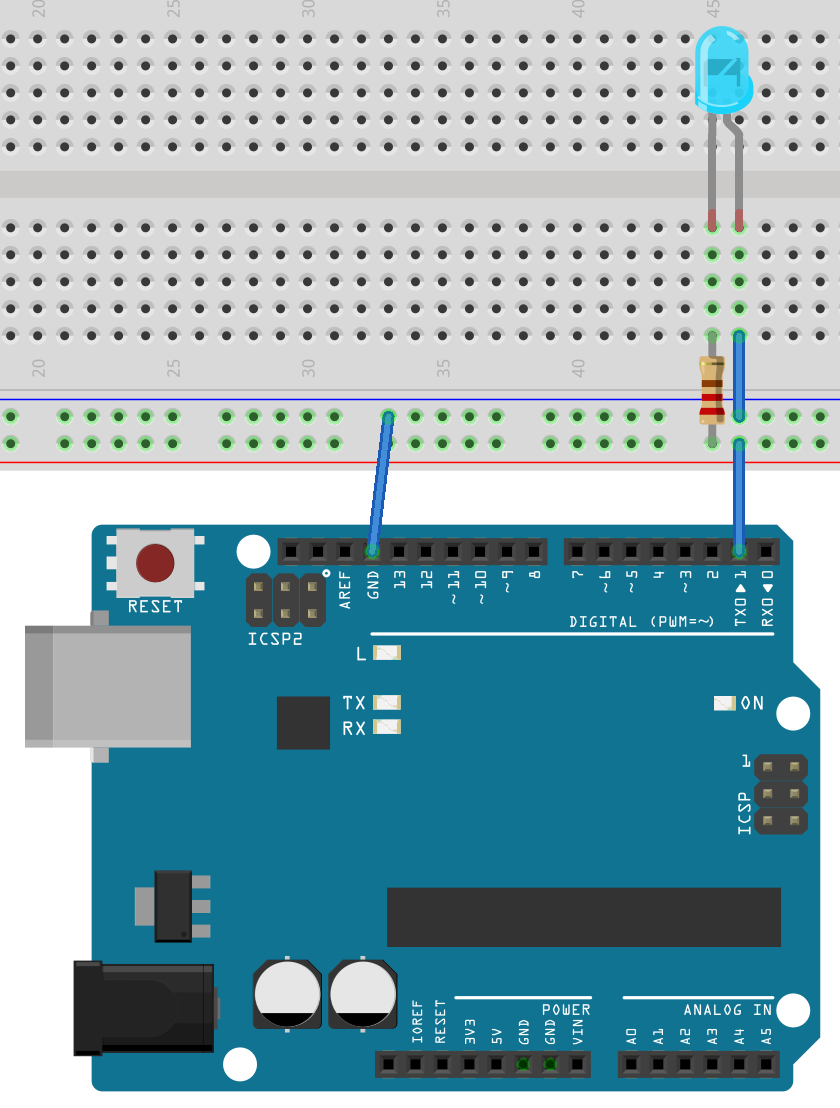
\includegraphics[width=\textwidth]{res/img/led}    
                \end{subfigure}
                \begin{subfigure}[b]{0.35\textwidth}
                    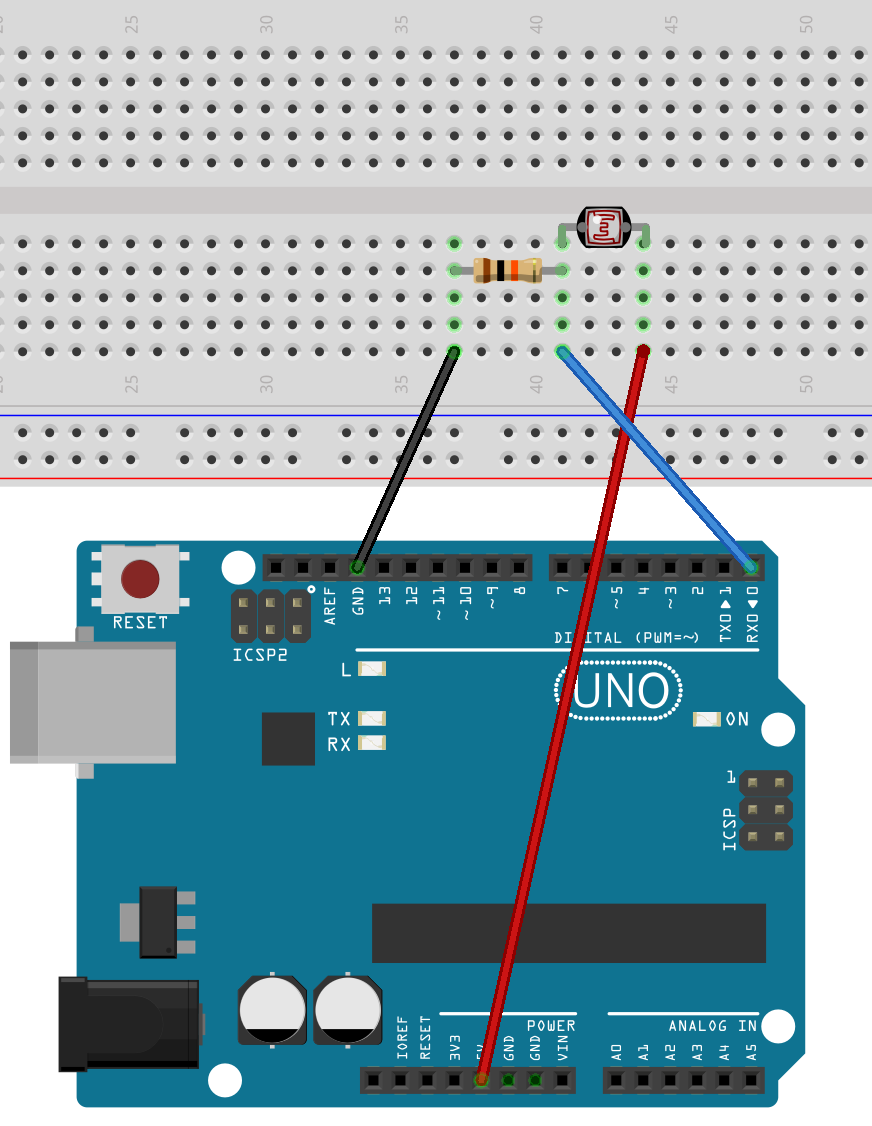
\includegraphics[width=\textwidth]{res/img/resistor}    
                \end{subfigure}
            \caption{Schema över sändare/mottagare}\label{fig:schema}
            \end{figure}

            Den andra lösningen använder sig endast av en lux-mätare upp på taket för att hämta in den data som efterfrågas. Genom att koppla samman två fibrer nere i rummet kommer ljuset att skickas upp till taket igen. För att nyttja den här metoden behöver samtliga linser som tillhör en fiberkabel täckas över på panelen, för att förhindra att solljus från ett dubbelt ljusintag transporteras i de båda fiberkablarna. Kablarna är anpassade för att hantera den värme som produceras av det ljus som normalt transporteras vid fullt dagsljus, skulle den dubbla mängden transporteras så riskerar fibrerna att smälta över överhettning. Den här lösningen använder sig inte av fiber som bärare av data utan endast av det solljus som panelen tar in, vilket minskar komplexiteten i systemet och minskar risken för störningar av data. 
            % subsection förutsättningar (end)

        \subsubsection{Tillförlitlighet} % (fold)
        \label{sub:tillf_rlitlighet}
            Genom att använda de fördragna fiberoptiska kablarna säkerställs att det ljus som skickas från rummet upp till panelen alltid kommer att levereras, förutsatt att ljuskällan är tillräckligt stark. Detta är i skarp kontrast mot en trådlös lösning, där flera lager betong mellan rummet och panelen inte är en osannolik företeelse vilket då skulle resultera att datan aldrig når till panelen.
        % subsection tillf_rlitlighet (end)
    % subsection optisk_kommunikation (end)

    \subsection{Applikation} % (fold)
    \label{sub:applikation}
        Sökalgoritmen implementerades i en Pythonapplikation med grafiskt gränssnitt och applikationen stödjer inhämtning av ljusvärden från antingen en till samma dator direkt ansluten luxmätare eller seriell mottagning från en annan enhet. Den luxmätare som användes vid implementationen av direkt anslutning var Yocto-Light-V3 medan Adafruit TSL2591 användes för avläsning som sedan överfördes seriellt via en Arduino Uno. Luxmätarna är beskrivna i avsnitt \ref{sub:yocto} respektive \ref{ssub:ada_tsl2591}. För seriell kommunikation använder applikationen sig av pySerial, ett bibliotek som kan hantera seriell kommunikation på de flesta vanligt förekommande operativsystem \cite{pyserial}. \bigskip

        Hos Parans finns sedan tidigare en Pythonapplikation med grafiskt gränssnitt anpassat till en pekskärm på en Raspberry Pi, där det grafiska gränssnittet är implementerat med biblioteket TkInter som medföljer standardinstallationer av Python \cite{solarremote}. TkInter och samma grafiska upplägg som tidigarenämnda applikation har använts till den applikation som utvecklats av projektet. Detta upplägg är tänkt att underlätta framtida hantering och utveckling av applikationerna och möjliggör en eventuell framtida integrering av de båda. \bigskip

        Applikationen har en modulär uppbyggnad och nya avläsningsmetoder kan implementeras utan större ingrepp i befintlig kod. Mjukvaran till Parans kommande solpanel, SP4, var ej färdigställd under projektets gång och således är applikationen riktad till SP3. Implementeringen av sökalgoritmen kan återanvändas till kommande versioner av solpaneler men vissa anpassningar kan behövas.
    % subsection applikation % (end)
% section resultat (end)
